\chapter{\introductionname}

Cuando en 1969, J. C. R. Licklider, un científico de la computación estadounidense, consiguió conectar el Instituto de Investigación de Stanford con la Universidad de California en Los Ángeles \cite{Rajaraman2022}, no podía imaginar en lo que llegaría a convertirse esa conexión. En ese momento, la idea de compartir recursos informáticos entre dos instituciones parecía revolucionaria, pero hoy en día, esa conexión es la base de lo que se conoce como Internet.

Desde entonces, Internet no ha hecho más que crecer y evolucionar, especialmente en los últimos años. Esto ha generado un interés creciente en mejorar la calidad del servicio (\textit{QoS}) optimizando aspectos como la latencia, el ancho de banda y la fiabilidad, pues Internet se ha convertido en una parte fundamental de las vidas y del trabajo de las personas. Sin embargo, cuanto más se usa Internet, más recursos se necesitan para mantenerlo funcionando, lo que ha llevado a un aumento en el consumo de energía y, por ende, a un impacto ambiental significativo.

Aunque parezca que la preocupación por las emisiones de carbono es algo reciente, la verdad es que lleva existiendo desde hace décadas. Por ejemplo, el 14 de marzo de 2001, el Parlamento Europeo adoptó una resolución sobre el impacto del consumo de energía y la necesidad de reducir este consumo en un 2.5\% anual, entre otras propuestas \cite{EuroparlTA52001141}. Otros estudios, como el de Paul J.M. Havinga y Gerard J.M. Smit \cite{Havinga2001}, han analizado el consumo de energía en redes inalámbricas y dispositivos móviles, destacando la importancia de la eficiencia en estos escenarios.

Uno de los grandes avances en redes que ha permitido mejorar la eficiencia energética es el desarrollo de las redes definidas por software (\textit{SDN}) \cite{Rout2021}. Las redes SDN y las redes tradicionales funcionan, esencialmente, de la misma manera: los dispositivos de red, como routers y switches, se encargan de dirigir el tráfico de datos hacia su destino. La diferencia fundamental entre ambos tipos de redes radica en cómo se gestionan y controlan estos dispositivos. En las redes tradicionales, cada dispositivo de red tiene integrado tanto el plano de control como el plano de datos, lo que significa que cada dispositivo toma sus propias decisiones sobre cómo manejar el tráfico. Por otro lado, las redes SDN separan el plano de control de los dispositivos y lo centralizan en lo que se denomina un controlador SDN. Este es el responsable de tomar decisiones sobre cómo debe dirigirse el tráfico y enviar estas intrucciones a los dispositivos de red, que se limitan a ejecutar las órdenes recibidas.

En la \autoref{fig:sdn_schema} se muestra un sencillo esquema de cómo funcionan las redes SDN. En este esquema, se puede observar cómo el controlador SDN se comunica con los dispositivos de red para indicarles cómo deben manejar el tráfico de datos. Si bien esta separación entre el plano de control y el plano de datos puede parecer un cambio menor, en realidad tiene un impacto significativo en la eficiencia energética de las redes. Al centralizar el control, las redes SDN pueden optimizar el uso de los recursos de red en función del algoritmo que esté ejecutándose en el controlador. Por ejemplo, si se quisiera reducir todo lo posible la carga de los enlaces, basta con definir e implementar un algoritmo que se centre en optimizar la redirección del tráfico para repartir equitativamente entre todos los enlaces todos los flujos de datos.

\begin{figure}[H]
    \centering
    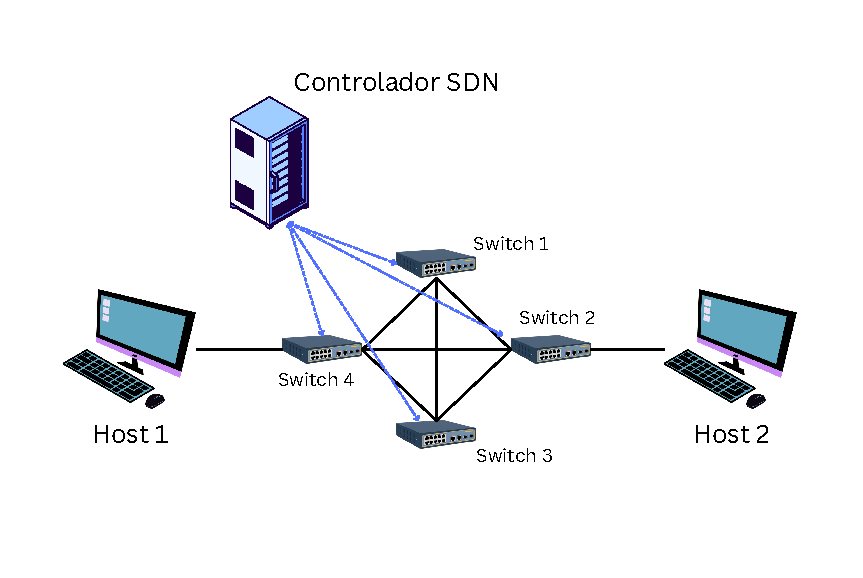
\includegraphics[width=0.7\textwidth]{pictures/sdn_schema.pdf}
    \caption[Esquema de redes SDN]{Representación gráfica de una red SDN.\\Fuente: Elaboración propia.}
    \label{fig:sdn_schema}
\end{figure}

El objetivo de este trabajo es reducir el consumo energético de las redes cableadas SDN mediante la implementación de un algoritmo de enrutamiento que optimice dicho consumo y, por ende, las emisiones de carbono. Existen dos perspectivas desde las que abordar este problema: apagar enlaces enteros o imponer restricciones en el ancho de banda de los enlaces. Aunque el segundo enfoque ofrece una mayor flexibilidad y potencialmente mejores resultados respecto al primer enfoque \cite{GomezdelaHiz2025}, también es más complejo de implementar. Este es el motivo por el cual se ha decidido centrarse en el apagado de enlaces.

Al estar hablando de un problema de optimización, existen muchas técnicas que podrían ser aplicadas para resolverlo. Como se busca una solución que ofrezca resultados lo suficientemente buenos en un tiempo razonable, las opciones a considerar se limitan bastante. En este caso, se ha optado por usar un algoritmo metaheurístico de optimización por enjambre de partículas (PSO), pues es un algoritmo que se ha demostrado eficaz en problemas de optimización similares y que, además, es relativamente sencillo de implementar. El algoritmo que finalmente se ha desarrollado se detalla en el \autoref{chp:implementacion}, mientras que en el \autoref{chp:results} se presentan los resultados obtenidos de las pruebas realizadas. Por otro lado, en el \autoref{chp:stateoftheart} se explican diferente conceptos y técnicas relacionados con el problema que se está tratando de resolver, mientras que en el \autoref{chp:metodologia} se detalla la metodología seguida para la realización de este trabajo. Finalmente, en el \autoref{chp:conclusiones}, se presentan las conclusiones que se han sacado en claro de las resultados obtenidos, así como las líneas de trabajo futuras que se podrían seguir a partir de este trabajo.